% =====================================================================
%  Strona tytułowa — tytuł, autor, wykres z podpisem.
% =====================================================================
\begin{titlepage}
\centering
\vspace*{1.0cm}

\slayertitle
  {Slayer 150 1.01:\\ wybór przepisu treningu przy regułach\\ ustalanych przed każdym wynikiem}%
  {Arkadiusz Słota, Fabryka AI}%
  {Wersja robocza, 7 października 2026 --- trening w toku}

\vspace{0.8cm}

\begin{figure}[h]
  \centering
  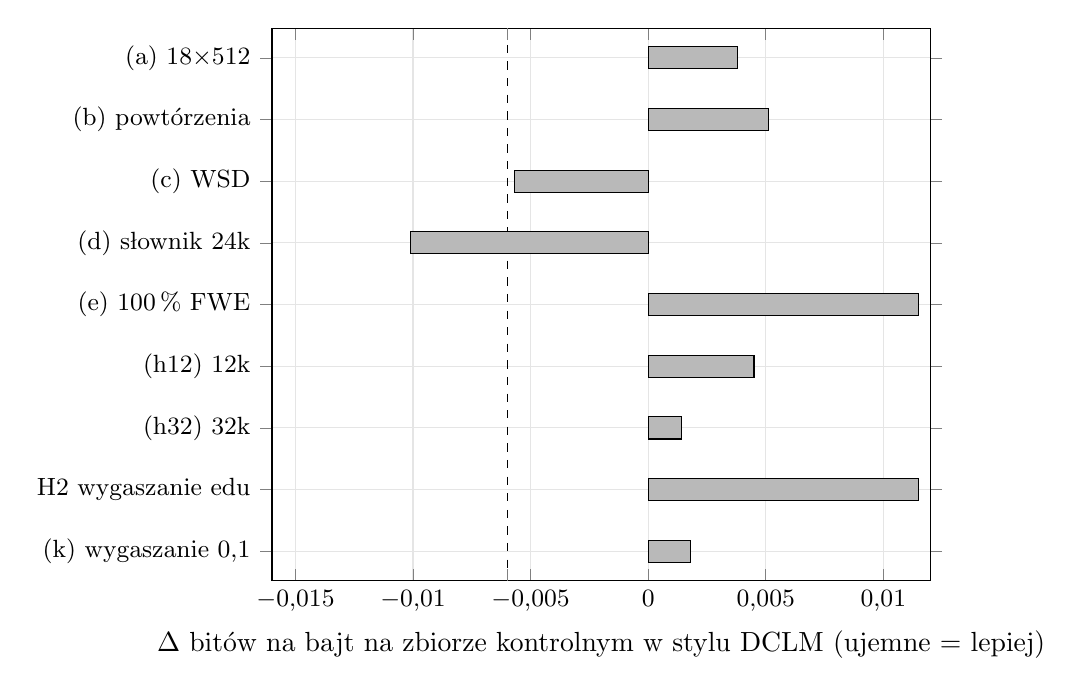
\begin{tikzpicture}
    \begin{axis}[
        xbar, width=0.82\linewidth, height=8.6cm,
        xlabel={$\Delta$ bitów na bajt na zbiorze kontrolnym w stylu DCLM (ujemne = lepiej)},
        xmin=-0.016, xmax=0.012,
        ytick={1,...,9},
        yticklabels={(a) 18$\times$512, (b) powtórzenia, (c) WSD, (d) słownik 24k, (e) 100\,\% FWE, (h12) 12k, (h32) 32k, H2 wygaszanie edu, (k) wygaszanie 0{,}1},
        scaled x ticks=false, xtick={-0.015,-0.010,-0.005,0,0.005,0.010},
        x tick label style={/pgf/number format/fixed, /pgf/number format/precision=3, /pgf/number format/use comma, font=\small},
        bar width=8pt, enlarge y limits=0.06,
        grid=major, grid style={gray!20},
        extra x ticks={-0.006}, extra x tick labels={}, extra x tick style={grid=major, grid style={black, dashed}},
        y dir=reverse, y tick label style={font=\small},
    ]
      \addplot[fill=gray!55] coordinates {
        (0.0038,1) (0.0051,2) (-0.0057,3) (-0.0101,4) (0.0115,5) (0.0045,6) (0.0014,7) (0.0115,8) (0.0018,9)};
    \end{axis}
  \end{tikzpicture}
  \caption{\textbf{Dziewięć ablacji (64M parametrów, 2 mld tokenów) ocenianych regułami zapisanymi przed każdym
  wynikiem.} Słupki pokazują zmianę liczby bitów na bajt na zbiorze kontrolnym w stylu DCLM wobec punktu
  odniesienia danego wariantu; linia przerywana to próg przyjęcia $-0{,}006$. Przekroczył go tylko słownik 24k (d).
  Słupki (e) i H2 są ucięte na $+0{,}0115$; prawdziwe wartości to $+0{,}0888$ i $+0{,}0505$. Wartości z plików
  werdyktów wymienionych w \texttt{recipe/}.}
  \label{fig:hero}
\end{figure}

\vfill
{\small Fabryka AI \textperiodcentered{} SlayerLabs \textperiodcentered{} wszystkie liczby przypięte skrótami SHA-256 do plików wyników}
\end{titlepage}
